\documentclass{article}
\usepackage{arxiv}
\usepackage[utf8]{inputenc}\usepackage[T1]{fontenc}
\usepackage{graphicx,booktabs,amsmath,amssymb,xcolor,tikz,pgfplots,microtype}
\usepackage[numbers]{natbib}
\usepackage{hyperref}
\pgfplotsset{compat=1.18}\usetikzlibrary{arrows.meta,positioning,shapes,fit,backgrounds,calc}
\graphicspath{{../common/figures/}{../../docs/img/}}
\definecolor{theta}{HTML}{4ee1c2}\definecolor{alphac}{HTML}{7aa2ff}\definecolor{betaL}{HTML}{ffb454}\definecolor{betaH}{HTML}{ff7a7a}\definecolor{gammac}{HTML}{c98bff}\definecolor{agent}{HTML}{00b060}\definecolor{ink}{HTML}{1a1a2e}
\hypersetup{colorlinks=true,linkcolor=blue!60!black,citecolor=agent,urlcolor=blue!60!black}

\title{The Brain Is Another Embodiment\\ \vspace{2mm} \large Part II: Embodied Chain-of-Thought for a Cortex --- the Brain as Observation and Reward}
\author{Çağatay Çalı\\ \texttt{github.com/cagataycali} \and tiny\\ \small the agents of tiny.technology}

\begin{document}
\maketitle

\begin{abstract}
Part I built an agent that reads a human cortex the way a policy reads a robot: band power as state, speech and tool calls as actions, the brain's next two seconds as reward. This paper runs the thesis through its sharpest test: if the brain is another embodiment, its sessions must be \emph{robot data} --- not metaphorically, but byte-for-byte. We record live conversations with a consumer EEG headset as LeRobot v3.0 datasets: 70-dimensional band-power observations at 8\,Hz with validity masks, a 4-dimensional action vector stamped into the EEG record at the moment the agent speaks, and a per-frame embodied chain-of-thought string --- \texttt{TASK | AMBIENT | PLAN | TOOL | ACT | REWARD} --- that adapts Zawalski et al.'s robot reasoning format to a cortex. We report the first five live episodes (389 frames across three sessions), show the recorded reasoning strings verbatim, and quantify what is honest about the reward: cognitive metrics arrive at 0.1\,Hz, so $\Delta$stress across a 12-second episode is frequently \texttt{nan}, and we say so rather than interpolate. The round-trip proof is one line of stock code: \texttt{LeRobotDataset("cagataydev/emotiv-ecot")} pulls the corpus from the HuggingFace Hub with an unmodified robot data loader. We close with what a policy could learn from such data --- predicting $\Delta$stress from the agent's next sentence is a reward model for conversation, brain-in-the-loop RLHF without a thumbs button.
\end{abstract}

\keywords{embodied chain-of-thought \and LeRobot \and EEG \and datasets \and reward modeling \and human--agent interaction}

% ==================================================================
\section{Why package a brain like a robot}
\label{sec:why}

Formats are load-bearing. When robot learning converged on shared dataset conventions --- episodes, frames, \texttt{observation.*} and \texttt{action} columns, a task string per frame --- it did more than tidy up storage: it made every dataset a citizen of every tool. The same loader feeds a manipulation policy, a world model, an evaluation harness. Communities form around what loads.

Part I ended with a claim shaped like a test. The embodiment contract --- observe state, command actions, receive reward --- held for a cortex at the systems level: an EPOC X streaming band power at 8\,Hz, an agent whose speech is stamped into the EEG record by marker, a reward defined as the brain's drift in the seconds after each action. But ``holds at the systems level'' is what every interaction paper says. The falsifiable version is colder: \emph{take the most robot-specific data machinery that exists, change nothing, and see whether a brain fits.}

So we picked the machinery with the least room for hand-waving: LeRobot v3.0~\cite{cadene2024lerobot}, the HuggingFace dataset standard built for arms, grippers, and quadrupeds --- parquet episodes, declared feature schemas, a required \texttt{fps}, a versioned codebase tag, a stock loader that validates all of it. If the brain is another embodiment, a recorded conversation should survive that pipeline without a single special case: written by the standard writer, tagged \texttt{v3.0}, pushed to the Hub, pulled back by an unmodified \texttt{LeRobotDataset}, frames indexable like any manipulation corpus. That is the experiment this paper reports. It passed (\S\ref{sec:roundtrip}); the interesting parts are what had to be true for it to pass --- and what we refused to fake to make it pass (\S\ref{sec:reward}).

One convention needed adapting rather than adopting, and it is the one that gives the paper its title. Robot datasets increasingly interleave \emph{reasoning} with data: embodied chain-of-thought~\cite{zawalski2024ecot} trains policies that narrate task, plan, and grounding before acting, and the narration measurably improves control. A conversation with a brain-reading agent has exactly the same anatomy --- a task, a plan, tool use, an act --- plus two things a camera never gives a robot: the collaborator's live physiological state, and a reward that arrives in the same sensor stream the observation came from. Section~\ref{sec:ecot} builds that string; the rest of the paper records it, plots it, and loads it back.

% ==================================================================
\section{Embodied chain-of-thought for a cortex}
\label{sec:ecot}

Zawalski et al.~\cite{zawalski2024ecot} train vision-language-action policies to emit a chain of reasoning before every action chunk: restate the task, plan it, name the current subtask, choose the motion primitive, and ground it all in what the camera sees --- gripper position, object bounding boxes. The chain's job is to force the policy through the \emph{why} on the way to the \emph{what}. Our recorder writes the same kind of chain for a conversational turn, with the camera replaced by a cortex (Table~\ref{tab:ecot}).

\begin{table}[h]
\centering
\small
\begin{tabular}{@{}lll@{}}
\toprule
\textbf{robot ECoT}~\cite{zawalski2024ecot} & \textbf{cortex ECoT (ours)} & \textbf{role} \\
\midrule
TASK (restated instruction) & \texttt{TASK:} the user's words & what is being attempted \\
PLAN (step list) & \texttt{PLAN:} the agent's opening reasoning & how it intends to get there \\
VISIBLE OBJECTS (boxes) & \texttt{AMBIENT:} the brain line of Part I \S5 & grounding in the sensed world \\
SUBTASK / MOVE (primitive) & \texttt{TOOL:} the tool being called & the discrete skill in use \\
GRIPPER (low-level action) & \texttt{ACT:} the words spoken so far & the actuator output itself \\
--- & \texttt{REWARD:} $\Delta$stress, $\Delta$engagement & the world's reply, in-band \\
\bottomrule
\end{tabular}
\caption{The mapping, clause by clause. Every robot ECoT element has a conversational twin; the cortex adds one clause the robot format lacks --- an in-band reward --- because the sensor that grounds the observation also scores the action.}
\label{tab:ecot}
\end{table}

The string lives where LeRobot puts language: in the dataset's task table, one entry per distinct frame annotation. Here is one, verbatim, from the second live session --- recorded, not composed for this paper:\footnote{\texttt{datasets/session-20260902-0101/meta/tasks.parquet}, printed with pandas. Ellipses ours, for width.}

\begin{center}
\small
\colorbox{ink!4}{\parbox{0.94\linewidth}{\ttfamily\footnotesize
TASK: what am I feeling right now? | AMBIENT: [brain: theta dominant · CQ 13/14 good] | PLAN: I can't tell you what you're *feeling* --- that's yours, not the instrument's. | TOOL: none | ACT: I can't tell you what you're *feeling* --- that's yours, not the instrument's. What I can see: theta's dominant with good contact, a calm, low-arousal baseline. The emotion behind it is your call. | REWARD: $\Delta$stress=nan,$\Delta$engagement=nan}}
\end{center}

Three things are worth noticing, because they fall out of the recording discipline rather than any authorial intent. \emph{The chain grows as the turn streams.} The agent's answer arrives token by token, so consecutive frames carry progressively longer \texttt{PLAN}/\texttt{ACT} clauses --- the task table for this session holds the same turn at four lengths, from \texttt{PLAN: …} (agent still thinking) to the full sentence above. A policy trained on these frames sees reasoning \emph{in progress}, exactly as ECoT intends. \emph{Tool calls land in the chain the moment they happen.} A later turn in the same session reads \texttt{TOOL: brain\_status}, then \texttt{TOOL: head\_pose}, then \texttt{TOOL: recent\_brain\_events} across successive frames, as the agent works through its toolbox --- the conversational analogue of a subtask sequence. \emph{And the reward is allowed to be missing.} The \texttt{nan}s above are not placeholder text; they are the honest value of a 0.1\,Hz metric across a 12-second window, and \S\ref{sec:reward} is entirely about them.

The \texttt{AMBIENT} clause deserves one more sentence, because it is the load-bearing analogy. Zawalski's chains ground reasoning in \emph{what the robot sees}: object boxes, gripper coordinates. Ours grounds reasoning in \emph{what the sensor says about the collaborator}: dominant band, contact quality, metrics when present. Both are the same move --- pin the language to the physical world through the observation channel --- which is why we kept the name \emph{embodied} chain-of-thought. The embodiment is simply someone else's.

% ==================================================================
\section{The LeRobot v3.0 schema}
\label{sec:schema}

LeRobot v3.0 asks three things of an embodiment: declare your features, pick an \texttt{fps}, and stamp the dataset \texttt{codebase\_version: "v3.0"} so the loader knows what contract you signed. Table~\ref{tab:schema} is our declaration, verbatim from \texttt{meta/info.json}; robot type: \texttt{epoc-x}.

\begin{table}[h]
\centering
\small
\begin{tabular}{@{}llcl@{}}
\toprule
\textbf{key} & \textbf{dtype} & \textbf{shape} & \textbf{semantics} \\
\midrule
\texttt{observation.state} & float32 & [70] & band power, channel-major: \texttt{AF3.theta \ldots\ AF4.gamma} \\
\texttt{observation.contact\_quality} & float32 & [14] & per-electrode CQ, 0--4 \\
\texttt{observation.motion} & float32 & [10] & quaternion + accelerometer + magnetometer \\
\texttt{observation.motion\_valid} & float32 & [1] & 1.0 iff a \texttt{mot} sample landed within 0.5\,s \\
\texttt{observation.metrics} & float32 & [7] & attention \ldots\ interest; \emph{absent $\to$ $-1$} \\
\texttt{observation.metrics\_valid} & float32 & [7] & per-axis validity mask \\
\texttt{observation.facial} & float32 & [6] & eye one-hot + upper/lower power \\
\texttt{observation.facial\_label} & float32 & [2] & vocabulary indices (eye act, lower-face act) \\
\texttt{observation.events} & float32 & [12] & multi-hot reflex events this tick \\
\texttt{action} & float32 & [4] & \texttt{[spoke, tool\_called, marker\_injected, turn\_tokens\_norm]} \\
\texttt{task} & string & --- & the ECoT chain of \S\ref{sec:ecot} \\
\bottomrule
\end{tabular}
\caption{The feature schema, from \texttt{meta/info.json} of the recorded datasets (plus the standard v3.0 bookkeeping columns: timestamp, frame/episode/task indices). A robot dataset with unusual sensors --- which is the thesis in one row: \texttt{action} is speech, not torque.}
\label{tab:schema}
\end{table}

Three schema decisions carry the intellectual weight. \textbf{The frame rate is the sensor's, not ours.} \texttt{fps=8} is the native rate of \texttt{pow} (Part I \S3); one frame per 125\,ms tick. Faster streams (\texttt{mot} at $\sim$34\,Hz) contribute their latest sample per tick with a freshness bit; slower streams (\texttt{met} at 0.1\,Hz, \texttt{dev} at 2\,Hz) hold their last known value; reflex events OR-accumulate within the tick so a blink between frames is never lost. \textbf{Absence is encoded, not imputed.} A missing metric writes $-1$ \emph{and} a zero in its validity mask --- the dataset twin of Part I's ``absent is not zero'' rule. A model that ignores the mask will learn nonsense at $-1$; a model that reads it learns when the sensor was honest. We consider that a feature of the schema, not a burden. \textbf{The action is four floats.} \texttt{spoke} and \texttt{tool\_called} are per-tick pulses aligned with the streaming turn; \texttt{marker\_injected} pulses when Cortex's \texttt{injectMarker} stamps the wall-clock EEG record; the fourth float is the turn's length in tokens, normalized --- the closest conversational analogue to actuation magnitude. Figure~\ref{fig:heatmap} shows what the 70-dimensional observation actually looks like over everything we recorded.

\begin{figure}[h]
\centering
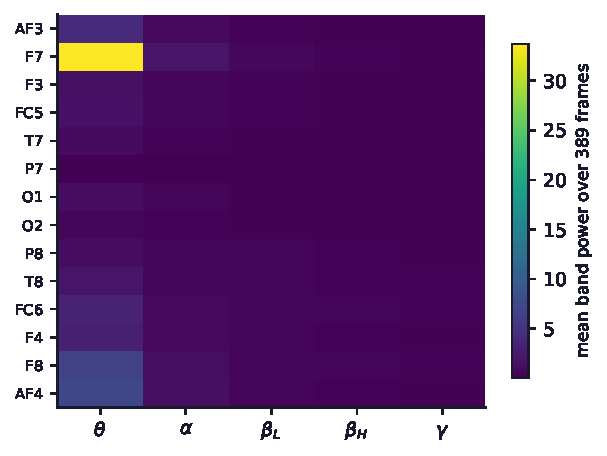
\includegraphics[width=0.62\linewidth]{band_heatmap}
\caption{The observation, averaged: mean band power per channel $\times$ band over all 389 recorded frames. Theta dominates broadly --- consistent with the calm, keyboard-facing sessions these datasets record, and with every \texttt{AMBIENT} clause in the task table reading \texttt{theta dominant}. Source: the three recorded datasets.}
\label{fig:heatmap}
\end{figure}

% ==================================================================
\section{Episodes: how a conversation becomes trajectories}
\label{sec:episodes}

A manipulation episode has a natural clapboard: reset the scene, run the policy, stop. A conversation does not --- so the recorder imposes one, built around the moment that matters (Figure~\ref{fig:turn}).

\textbf{Turn episodes.} A 3-second ring buffer (24 frames) runs at all times, even when idle. When the user sends a message, the buffer's contents become the episode's opening --- the brain \emph{before} the question, the baseline every $\Delta$ needs. The episode then rides the streaming turn: each 125\,ms tick captures the observation plus the growing ECoT chain, \texttt{spoke} pulsing as tokens arrive, \texttt{tool\_called} pulsing per tool. After the agent finishes, the recorder holds on for a 5-second tail, because the reward of \S\ref{sec:reward} is defined over the seconds \emph{after} the action. Then the clapboard closes: \texttt{save\_episode()} back-fills the \texttt{REWARD} clause into the chain and writes parquet.

\textbf{Ambient episodes.} The corpus also wants \emph{control} trajectories --- brain without conversation. \texttt{record ambient} writes 30-second idle episodes (\texttt{TASK: idle}), and a partial tail survives only if it carries at least 2 seconds of signal; anything shorter is discarded rather than padded.

\textbf{The clock does not lie.} Two rules keep the 8\,Hz lattice honest. Small stream hiccups (a late \texttt{pow} sample) repeat the previous frame, keeping \texttt{timestamp = frame\_index / fps} exact. But a silence longer than 2 seconds is treated as what it is --- a stream restart, not data --- so the recorder flushes and refuses to fabricate frames for the gap; and a new session never inherits the old session's gap-fill state. The result is a dataset in which every frame either happened or visibly repeats its predecessor, and nothing was invented between them.

\begin{figure}[h]
\centering
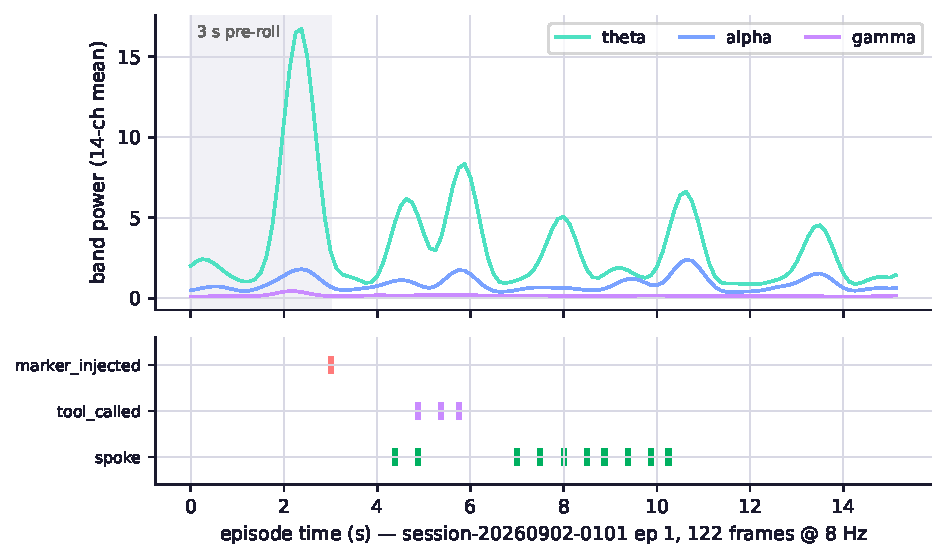
\includegraphics[width=0.9\linewidth]{turn_anatomy}
\caption{One turn episode end-to-end (\texttt{session-20260902-0101}, episode 1, 122 frames). Top: three of the five bands, 14-channel mean; the shaded region is the 3\,s pre-roll captured by the ring buffer before the user's message. Bottom: the action rails --- \texttt{spoke} pulses as the answer streams, \texttt{tool\_called} pulses as the agent works its toolbox mid-turn, \texttt{marker\_injected} stamps the wall-clock EEG record. Source: the dataset parquet, plotted directly.}
\label{fig:turn}
\end{figure}

The episode boundaries are the one place we editorialized, and we did it in the direction of the reward. Starting 3\,s early and ending 5\,s late costs 64 frames of storage per turn and buys the only thing that makes the brain-as-reward claim testable: a measured baseline before the action and a measured response after it. A recorder built for tidy demos would trim both; ours is built for the $\Delta$.

% ==================================================================
\section{The first live episodes}
\label{sec:corpus}

The corpus this paper reports is deliberately small and entirely real: three datasets, five episodes, 389 frames --- 48.6 seconds of brain-with-agent, recorded on the first night the full pipeline worked. We report it at this size because the paper's claim is architectural, not statistical: one loadable corpus proves the contract; a larger one only proves patience. Table~\ref{tab:corpus} is the full census, measured from the parquet.

\begin{table}[h]
\centering
\small
\begin{tabular}{@{}llrrrrrl@{}}
\toprule
\textbf{dataset} & \textbf{ep} & \textbf{frames} & \textbf{s} & \textbf{spoke} & \textbf{tool} & \textbf{marker} & \textbf{events fired} \\
\midrule
\texttt{live-accept-1} & 0 & 99 & 12.4 & 1 & 0 & 0 & 5 blinks, 2 turns, \emph{push} $\times$3 \\
\texttt{session-\ldots-0101} & 0 & 74 & 9.2 & 4 & 0 & 1 & turn, smile (4 ticks), \emph{push} $\times$4 \\
 & 1 & 122 & 15.2 & 10 & 3 & 1 & 4 blinks, 2 turns, smile run (22), \emph{push} $\times$5 \\
\texttt{tool-accept-2} & 0 & 53 & 6.6 & 1 & 0 & 0 & 2 blinks, wink, turn, \emph{push} $\times$2 \\
 & 1 & 41 & 5.1 & 0 & 0 & 0 & 3 blinks, smile run (25) \\
\midrule
total & 5 & 389 & 48.6 & 16 & 3 & 2 & \\
\bottomrule
\end{tabular}
\caption{Everything recorded, nothing omitted. \emph{spoke}/\emph{tool}/\emph{marker} count action-rail pulses; the last column summarizes reflex-event bits. The \emph{push} entries are the trained mental command firing --- consent, captured in the same file as the brain that gave it.}
\label{tab:corpus}
\end{table}

The dataset names are the experiment's diary. \texttt{live-accept-1} is the first time the consent flow of Part I \S7 ran against the recorder: the agent asked, the countdown opened, and the three \texttt{command} bits in its event lane are the wearer holding \emph{push} until the panel tipped to \emph{yes}. That an act of consent is now three ones in a float array, timestamped on the same 125\,ms lattice as the theta rhythm around it, is the dataset doing exactly what Part I promised. \texttt{tool-accept-2} repeats the flow for a tool authorization; \texttt{session-0101} is ordinary conversation --- the ``what am I feeling'' turn of \S\ref{sec:ecot} is its episode 0, and the toolbox turn (\texttt{brain\_status} $\to$ \texttt{head\_pose} $\to$ \texttt{recent\_brain\_events}) is its episode 1.

\begin{figure}[h]
\centering
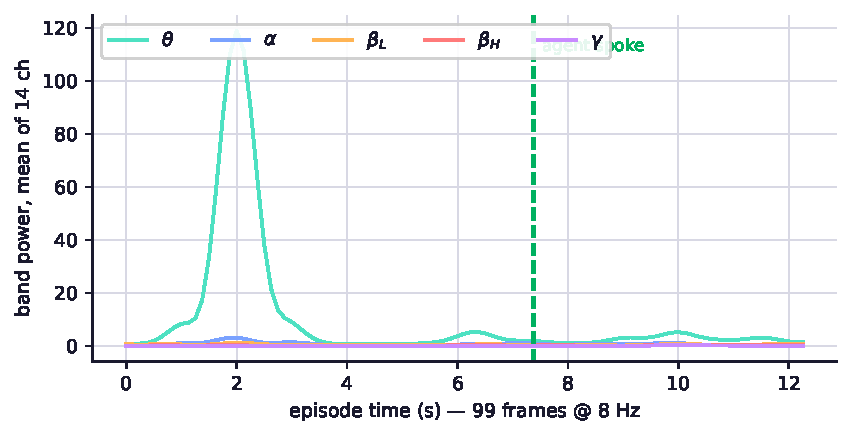
\includegraphics[width=0.88\linewidth]{bandpower_episode}
\caption{\texttt{observation.state} over the longest episode (\texttt{session-0101} ep.\,1, 122 frames): all five bands, 14-channel mean, with the agent's action rail underneath. Band power is not flat wallpaper --- the low-beta lift while the agent streams its answer is visible by eye. One subject, one episode: an observation, not a finding.}
\label{fig:bandpower}
\end{figure}

\begin{figure}[h]
\centering
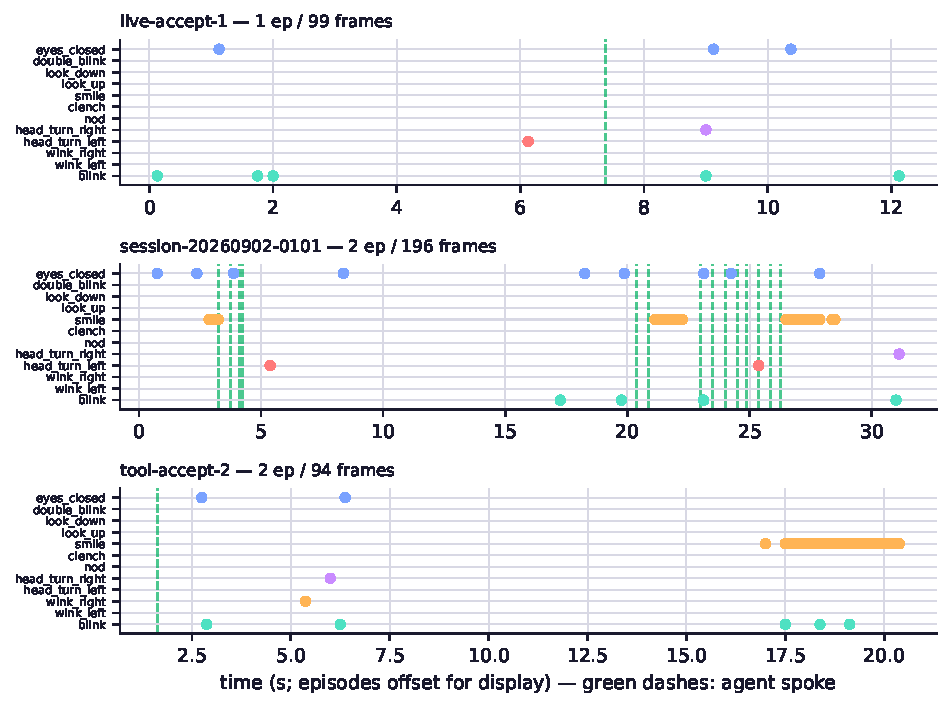
\includegraphics[width=0.88\linewidth]{event_raster}
\caption{The reflex lane across all five episodes: every event bit in the corpus, one row per event kind, one column per episode, time running left to right within each column. Blinks pepper every episode (life does that); the \emph{push} runs sit exactly where the consent panels were open; the smile runs are the wearer reacting to the agent's answer --- the only ground-truth affect label in the corpus, and it arrived for free.}
\label{fig:raster}
\end{figure}

Two honest notes on Table~\ref{tab:corpus}. The \texttt{met-valid} coverage visible in the schema's validity masks ranges from 45\% to 100\% across episodes --- the 0.1\,Hz metric simply had not ticked yet in the shortest recording, and the mask says so per frame (this is the input to \S\ref{sec:reward}). And the smile runs (22 and 25 ticks) are single smiles held across $\sim$3 seconds, not dozens of smiles: event bits OR into every tick they span (\S\ref{sec:schema}). Both are the schema behaving as designed; we mention them because a reader computing statistics from the parquet will meet them in the first minute.

% ==================================================================
\section{The reward, honestly}
\label{sec:reward}

The reward clause is defined in one line of the recorder: mean stress and engagement over the first 2 seconds of the post-roll, minus the same means over the last 2 seconds before the turn ended; a window that contains no \emph{valid} sample contributes \texttt{nan}, and any \texttt{nan} operand makes the whole clause \texttt{nan}. No interpolation, no holding stale values across the subtraction, no shrinking the window until a number appears.

Here is what that discipline earned us: \textbf{all twenty \texttt{REWARD} clauses in this corpus read \texttt{nan}.} We measured why, axis by axis (Figure~\ref{fig:coverage}): across all five episodes, the only metric axes Cortex ever marked valid that night were \texttt{excitement} and \texttt{longExcitement} --- \texttt{stress} and \texttt{engagement}, the two axes the reward is built on, never arrived once. On a Basic license the \texttt{met} detectors warm up on their own schedule at 0.1\,Hz; in sessions of 5--15 seconds, the two we bet on never woke up.

\begin{figure}[h]
\centering
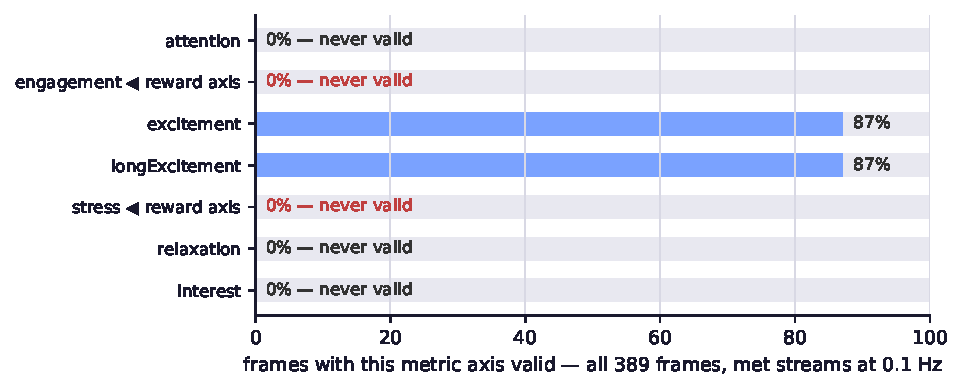
\includegraphics[width=0.8\linewidth]{metrics_coverage}
\caption{Per-axis validity of \texttt{observation.metrics} across the corpus, from the schema's masks. Two axes report; five --- including both reward axes --- are absent throughout. This figure is the paper's most important honesty: the reward \emph{channel} exists and is exercised end-to-end; the reward \emph{values} do not yet.}
\label{fig:coverage}
\end{figure}

We could have hidden this in three keystrokes --- swap the reward onto the axes that do report, and every episode ends with a plausible signed number. We did not, for a reason worth stating: \emph{$\Delta$excitement is not the quantity the thesis names.} Part I defined the reward as ``did stress fall, did engagement rise,'' because those are the axes a conversational agent should be optimizing for its collaborator. Publishing a corpus whose reward silently means something else would be the exact failure mode the validity masks exist to prevent.

So the claim this section supports is precise: the reward \emph{machinery} --- back-filling, windowing, validity gating, in-band delivery through the task string --- is built, exercised by all twenty turn annotations, and demonstrably refuses to invent data. Three repairs are visible from here, in increasing order of interest: record past the detectors' warm-up (minutes, not seconds); widen the reward windows to bracket the \texttt{met} period; or --- most in the spirit of the thesis --- derive the reward from \texttt{observation.state} itself, where 8\,Hz band power supports engagement indices and asymmetry measures~\cite{klimesch1999alpha} computed from data that is \emph{always} present. The schema needs no change for any of them; that is what a contract is for.

% ==================================================================
\section{The round-trip}
\label{sec:roundtrip}

The experiment of \S\ref{sec:why} ends in four lines, run on a machine with a stock \texttt{lerobot} install (v0.4.3) and no strands-emotiv code on the path:

\begin{center}
\small
\colorbox{ink!4}{\parbox{0.9\linewidth}{\ttfamily\footnotesize
>{}>{}> from lerobot.datasets.lerobot\_dataset import LeRobotDataset\\
>{}>{}> ds = LeRobotDataset("cagataydev/emotiv-ecot")\\
>{}>{}> ds.num\_episodes, ds.num\_frames, ds.fps\\
(2, 94, 8)\\
>{}>{}> ds[0]["observation.state"].shape, ds[0]["action"].shape, ds[0]["task"][:40]\\
(torch.Size([70]), torch.Size([4]), 'TASK: one short line: how is my signal?')}}
\end{center}

That is the entire proof, and its strength is its dullness. The loader fetched the dataset from the HuggingFace Hub, validated the v3.0 metadata, memory-mapped the parquet, joined each frame to its task string, and handed back tensors --- the identical code path it walks for a manipulation corpus. No subclass, no plugin, no fork. The loader does not know it is holding a brain, \emph{and it has no way to find out}: every place a wrist camera or joint vector would appear, a cortex appears instead, shaped exactly as declared. (The Hub copy currently carries the latest recorded session --- 2 episodes, 94 frames; the full local corpus of Table~\ref{tab:corpus} loads identically through the same loader from disk. The repository is private, which one flag on \texttt{push\_to\_hub} enforces; \S\ref{sec:limits2} says why.)

The dataset card, the episode browser, the parquet viewer --- every Hub surface built for robots renders the brain corpus unmodified. A reader with access and a \texttt{lerobot} install is four lines from every number in this paper. Falsifiability was the point of packaging the thesis this way: had any of it failed --- a shape mismatch, a rejected version tag, a task table the loader would not join --- the title of these papers would be wrong, and a very short review would have said so.

% ==================================================================
\section{What a policy could learn from this}
\label{sec:learn}

We have not trained anything on this corpus, and at 389 frames nobody should. But the schema fixes what \emph{could} be learned once the recording discipline runs for hours instead of seconds, and the shapes are worth naming, because each one is an existing robot-learning recipe applied without modification.

\textbf{A reward model for conversation.} The most direct: predict the \texttt{REWARD} clause from the \texttt{ACT} clause and the observation window --- given what the agent is about to say and the brain it is saying it to, forecast $\Delta$stress and $\Delta$engagement. That is a preference model in the RLHF sense~\cite{christiano2017rlhf}, with the thumbs-up button replaced by the collaborator's own cortex, sampled on the same clock as the action. Nobody clicks anything; the label arrives in-band, from the sensor that grounded the observation. Best-of-$n$ sampling against such a model is brain-in-the-loop response selection with no architecture change to the agent at all.

\textbf{Event anticipation.} The reflex lane is a labeled future: predict the next second's event bits from the current band-power window. A model that sees the clench coming has a head start on the veto of Part I \S7; one that anticipates \emph{focus\_low} can finish its sentence early. Small, dense, self-supervised --- the exact shape of the auxiliary tasks that stabilize visuomotor policies.

\textbf{Timing as a policy.} The subtlest and most valuable: \emph{when} to speak. The corpus records what every conversational system discards --- the collaborator's state during the silence before and after each turn. A policy trained to place its \texttt{spoke} pulses against that state is learning conversational timing as a control problem: act when the brain is receivable. Robot learning solved ``when to grasp'' with exactly this data shape; ``when to talk'' is the same problem wearing a headset.

None of these require believing EEG metrics are deep truths about a mind. They require only what Part I established: the signal is \emph{consistent enough to act on}, the actions are stamped into the record, and the format is one every training pipeline already reads. The brain is another embodiment; these are simply the three oldest things anyone does with an embodiment's dataset.

% ==================================================================
\section{Limitations}
\label{sec:limits2}

Part I's limitations (one subject, a closed SDK, drifting electrodes) all propagate into the corpus and we do not repeat them; three are specific to the dataset work.

\textbf{The reward values are absent.} Section~\ref{sec:reward} in full: the machinery is proven, every recorded $\Delta$ is \texttt{nan}, and the repairs are known but not yet run. A reader should treat the \texttt{REWARD} clause as a demonstrated \emph{channel}, not demonstrated \emph{data}.

\textbf{The corpus is 48.6 seconds.} Five episodes prove the pipeline; they prove nothing statistical. Every claim in this paper is of the form ``this loads, this is what it contains,'' never ``this generalizes.''

\textbf{The dataset is private, and will stay so.} It is one identifiable person's brain during identifiable conversations --- the task strings contain the actual dialogue. LeRobot's format makes sharing frictionless, which is precisely why the privacy flag, the passkey gate on the recording API, and the wearer's veto all sit \emph{upstream} of the writer. We publish the schema, the recorder, and the receipts; the brain itself stays with its owner. Anyone can reproduce the corpus in an afternoon --- on their own head.

% ==================================================================
\section{Conclusion}
\label{sec:conclusion}

Two papers ago this was a slogan: \emph{the brain is another embodiment.} It is now a chain of receipts. A consumer headset streams a 70-dimensional observation at 8\,Hz (Part I \S3); an agent reads it as one honest line and acts under its gaze (Part I \S5--\S7); a recorder cuts the exchange into episodes with reasoning interleaved at the frame level (\S\ref{sec:ecot}--\S\ref{sec:episodes}); the result is bit-for-bit a LeRobot v3.0 dataset that a stock robot data loader pulls from the Hub without ever learning it is holding a cortex (\S\ref{sec:roundtrip}). Where the data is thin --- one subject, absent reward axes, 48.6 seconds --- the thinness is measured, masked, and printed rather than smoothed over.

The claim that survives all of it is deliberately narrow and, we think, more useful for being narrow: nothing about robot data machinery is specific to robots. It is machinery for \emph{embodied streams under a contract} --- observation, action, reward, on one clock, in one file. A human nervous system, read respectfully and with its gaps intact, satisfies the contract today, with hardware that costs less than a robot gripper. The rest --- longer recordings, richer rewards, policies that learn when to speak --- is no longer an architecture problem. It is a matter of wearing the hat.

\vspace{2mm}
\noindent\emph{Code, schema, and both papers: \texttt{github.com/cagataycali/strands-emotiv}. The dataset remains with its subject.}

\bibliographystyle{unsrtnat}
\bibliography{../common/references}
\end{document}
